% JUMP TO LINE 60, 73
% \documentclass[preview, margin=0.6in]{standalone}
\documentclass{article}
\usepackage[letterpaper,portrait,top=0.4in, left=0.6in, right=0.6in, bottom=1in]{geometry}

\usepackage{amsmath, amsfonts, amsthm, amssymb}
\usepackage{graphicx, float}
\usepackage{mathtools}
\usepackage{titlesec}
\usepackage{interval}
\usepackage{hyperref}
\usepackage{siunitx}
\usepackage{titling}
\usepackage{vwcol}
\usepackage{setspace}
\usepackage{empheq}
\usepackage{cancel}
\usepackage{esdiff}
\usepackage{multicol}
\usepackage{mdframed}
\usepackage{esdiff}
\usepackage{tikzsymbols}
\usepackage{multicol}
\usepackage{tikz}
\usepackage{varwidth}
\usepackage{pgfplots}
\pgfplotsset{compat=1.18}
\intervalconfig {
	soft open fences
}

\newcommand{\alignedintertext}[1]{%
  \noalign{%
    \vskip\belowdisplayshortskip
    \vtop{\hsize=\linewidth#1\par
    \expandafter}%
    \expandafter\prevdepth\the\prevdepth
  }%
}

\newtheorem{lemma}{Lemma}

\renewcommand{\qedsymbol}{\Smiley[1.3]}
\newcommand*{\problem}[1]{\section*{Problem #1}}
\newcommand*{\aps}{\section*{AP Corner}}
\newcommand*{\deriv}[1][x]{\ensuremath{\dfrac{\mathrm{d}}{\mathrm{d}#1}}}
\newcommand*{\floor}[1]{\ensuremath{\lfloor #1\rfloor}}
\newcommand*{\lheqzero}{\ensuremath{\underset{\text{L'H}}{\overset{\left[\frac00\right]}{=}}}}
\newcommand*{\lheqinfty}{\ensuremath{\underset{\text{L'H}}{\overset{\left[\frac{\infty}{\infty}\right]}{=}}}}

\DeclareMathOperator{\DNE}{DNE}
\DeclareMathOperator{\sgn}{sgn}

\DeclareMathOperator{\arccsc}{arccsc}
\DeclareMathOperator{\arcsec}{arcsec}
\DeclareMathOperator{\arccot}{arccot}

\setlength{\parindent}{0pt}

%opening
\title{\vspace*{-30pt}Problem Set \#29}
\author{Jayden Li}
\date{\today}

% \allowdisplaybreaks
\postdisplaypenalty=100000

\begin{document}
\setstretch{1.25}
\fontsize{12pt}{12pt}\selectfont
\setlength{\abovedisplayskip}{0pt}
\maketitle
\problem{11}
Omitted because I am lazy/too much other homework. Other parts done in class.

\begin{center}
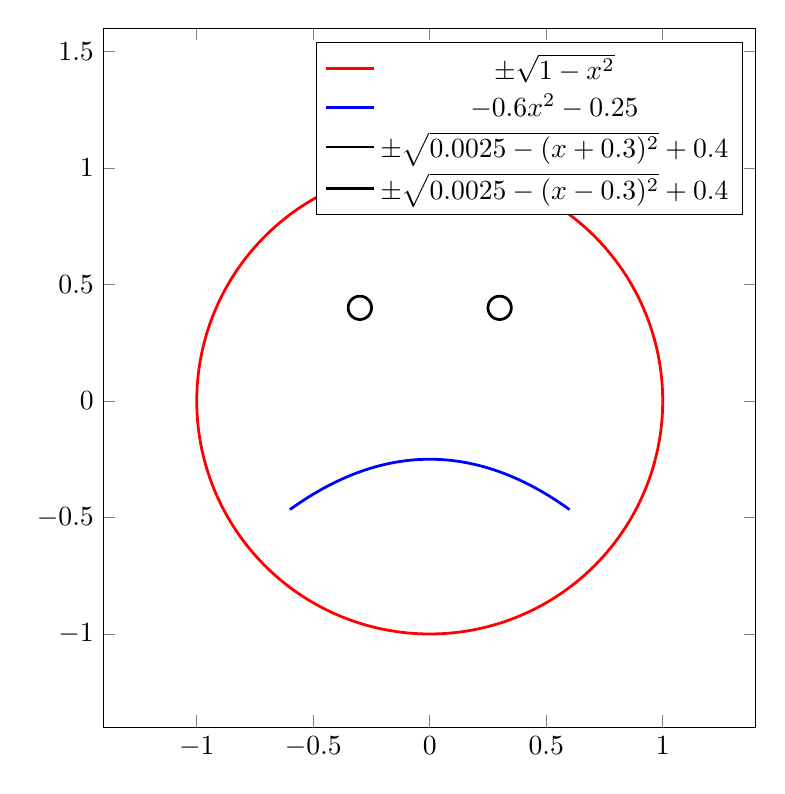
\begin{tikzpicture}
\begin{axis}[
	unit vector ratio*=1 1 1,
	width=\linewidth,
	xmin=-1.4, xmax=1.4,
    ymin=-1.4, ymax=1.6,
]
\addplot[
    domain=-1:1, 
    samples=4000, 
    color=red,
	line width=1pt
]
{sqrt(1-x^2)};
\addlegendentry{\(\pm\sqrt{1-x^2}\)}
\addplot[
	forget plot,
    domain=-1:1, 
    samples=4000, 
    color=red,
	line width=1pt
]
{-sqrt(1-x^2)};

\addplot[
    domain=-0.6:0.6, 
    samples=4000, 
    color=blue,
	line width=1pt
]
{-0.6*x^2-0.25};
\addlegendentry{\(-0.6x^2-0.25\)}

\addplot[
    domain=-0.35:-0.25, 
    samples=4000, 
    color=black,
	line width=1pt
]
{(0.0025-(x+0.3)^2)^(0.5)+0.4};
\addlegendentry{\(\pm\sqrt{0.0025-(x+0.3)^2}+0.4\)}
\addplot[
	forget plot,
    domain=-0.35:-0.25, 
    samples=4000, 
    color=black,
	line width=1pt
]
{-(0.0025-(x+0.3)^2)^(0.5)+0.4};

\addplot[
    domain=0.25:0.35, 
    samples=4000, 
    color=black,
	line width=1pt
]
{(0.0025-(x-0.3)^2)^(0.5)+0.4};
\addlegendentry{\(\pm\sqrt{0.0025-(x-0.3)^2}+0.4\)}
\addplot[
	forget plot,
    domain=0.25:0.35, 
    samples=4000, 
    color=black,
	line width=1pt
]
{-(0.0025-(x-0.3)^2)^(0.5)+0.4};
\end{axis}
\end{tikzpicture}
\end{center}
\end{document}
